\section{Usage} \label{sec:usage}

\paragraph{Topology File Parser Library} 
The topology file parser is a library that can be used to read and write files in the topology file format.  The 
files are built in an XML-like fashion and are implemented as a series of handles.  Below is a list of
the code in the source directory along with a description of the basic functionality each file provides. 
\begin{description}
\item[FileElement.h:] an abstract base class for reading and writing data.
\item[FileHandle.h:] the common base class for all file handles.
\item[DataHandle.h:] an overloaded file handle that can store an array of data.
\item[StatHandle.h:] an instance of DataHandle that stores per feature information.
\item[AttributeHandle.h:] an instance of StatHandle for per-feature attributes.
\item[AggregateHandle.h:] an instance of StatHandle for pre-accumulated attributes.
\item[SimplificationHandle.h:] an instance of DataHandle that stores the simplification sequence.
\item[ClanHandle.h:] an intance of FileHandle that encapsulates the functionality at the clan level. 
\item[FamilyHandle.h:] an instance of FileHandle that provides an interface to create and read handles for the different handle types.
\item[IndexHandle.h:] an instance of DataHandle that provides functionality for the per-feature index map.
\item[FeatureElement.h:] an instance of a FileElement that provides a bare-bones interface to a feature of a feature family.
\item[Feature.h:] an instance of a FileElement that provides an implmentation of a feature.
\item[FeatureHierarchy.h:] Feature hierarchy describes a hierarchical feature graph.
\end{description}

\paragraph{Statistics Browser} 
The Statistics Browser can be run by typing 

\texttt{\% ./gui/plot --i datafile.txt}

from the build directory where datafile.txt is a file whose first line is an integer specifying the number of files
to be loaded followed by the paths to the family files to be loaded.

\begin{figure}[h]
  \center
  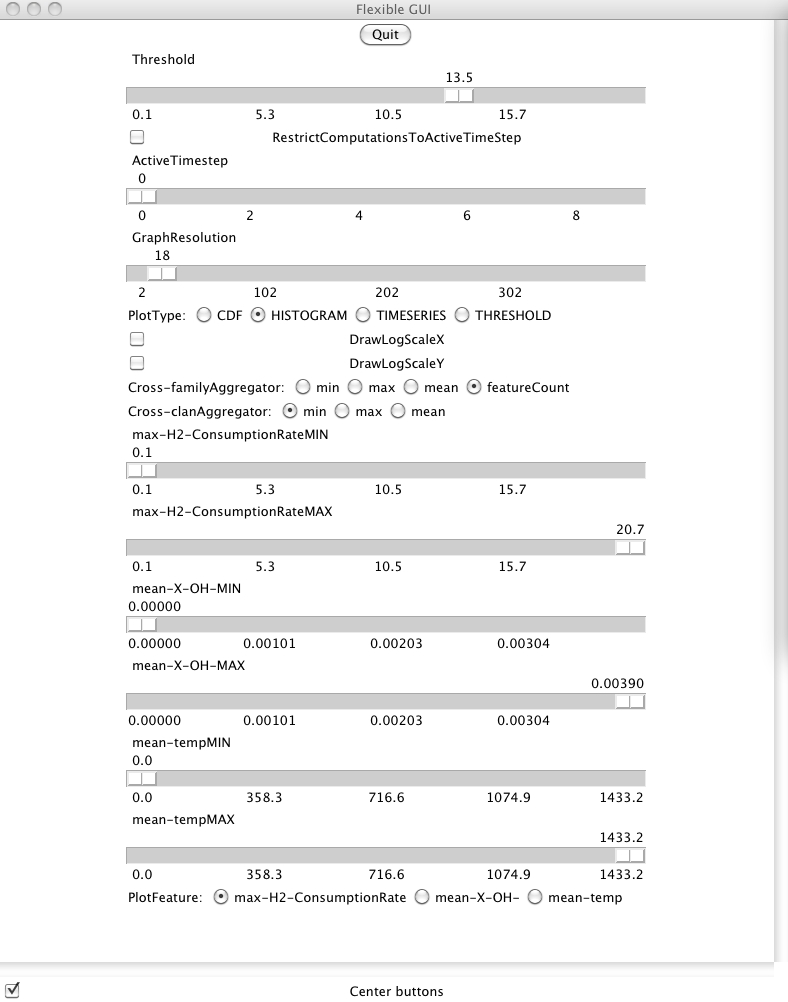
\includegraphics[width=5in]{jpeg/flexGUI.jpg} 
  \caption{The flexible user interface used by the Statistics Browser to control the state of the plots.}
  \label{fig:flexGUI}
\end{figure}

When the browser is run with this option a text file called \texttt{flexgui\_opt.txt} will be generated
in the build directory.  This file will contain a list of the available feature attributes for the data that has 
been loaded.  Next to each feature attribute will be a 0, because by default no feature attribute data is loaded.
You can load data associated with a feature by changing the value next to it to 1 and re-saving the file.
Attributes can be loaded and unloaded at any time.  Moreover, an initial option file can be specified at startup
to indicate which attributes should be loaded initially.  This is done with the command line option:

\texttt{--option\_file <name of file> }

An initial threshold value can also be specified by typing 

\texttt{--threshold <value> }

Upon startup two windows will appear as seen in figures \ref{fig:flexGUI} and \ref{fig:statsBrowser}. The Flexible GUI 
is updated automatically according to the attributes that have been loaded by the user.
It contains various buttons and sliders to control the state of the plots.  These are discussed in the
following as they appear from top to bottom in the GUI.  The threshold slider is used to specify 
a threshold value for the simplification hierachy and affects the CDF, histogram and time plots.  
There is a checkbox which allows you to restrict the computations to the active timestep.
When this checkbox is not selected the CDF and histogram are computed by evaluating features
over all timesteps.  However, when selected, CDFs and histograms are computed using features from
the active timestep only (as indicated by the active timestep slider). Graph resolution
affects the bucket sizes used for histograms and CDFs, and also indicates the number
of differet threshold samples used to create the threshold parameter plots.
Plot type is specified by radio buttons and the axes of the plots can be presented in log scale
if the associated checkboxes are checked.  There are radio buttons to spcify the Cross-family 
aggregator, which is a reduction operator across all time steps used by both the time plots and the 
parameter plots.  In addition to min, max and mean, feature count can be used as a cross-family
aggregator (a sample time plot using the feature count cross family aggregator would be a plot
of feature count vs time).  Cross clan aggregators are reduction
operators used by the threshold parameter plots only and at this time min, max, and mean are the 
only cross clan aggregators supported. The Flexible GUI contains a pair of sliders
for each feature attribute that has been loaded.  These sliders allow the user to subselect features
for analysis according to a function range.  Note that mean x, mean y and mean z values are often
stored with the feature families so that the sliders can be used to subselect features according to
their spatial location.   Finally, at the bottom of the Flexbile GUI there is a series of radio buttons
which are used to specify the plot attribute of interest for the current plot.  Note that when \emph{no
data is loaded} there will not be any sliders used for filtering or plot feature attribute radio buttons.
This means, that when loading the data for the first time, or if you are not providing an
--option\_file, you must modify the \texttt{flexgui\_opt.txt} to load data in order to generate a plot.

The Statistics Browser itself contains a display window for the plots.  Additionally, there are buttons to 
save active plots, clear saved plots, and clear the sub-selected feature ids so that all features are active 
again (i.e. this removes the effect of the sub-selection sliders in the Flexible GUI as well as direct plot selection, described shortly).
A filename can be specified and all saved plots can be written out in gnuplot file format (with a .plt file extension).  
Associated gnuplot data files are stored with the .dat file extension.  You can run gnuplot with your file as input (\url{http://www.gnuplot.info}).
to generate a postscript version of your plot.  

Note that by default the plot browser is automatically updated according to changes in the Flexble GUI, however an 
  option is provided in the Statistics Browser which allows the user to manually update the plot state after a set of multiple
  changes has been made.  This option can be useful when working with large data sets.

\begin{figure}[h]
  \center
  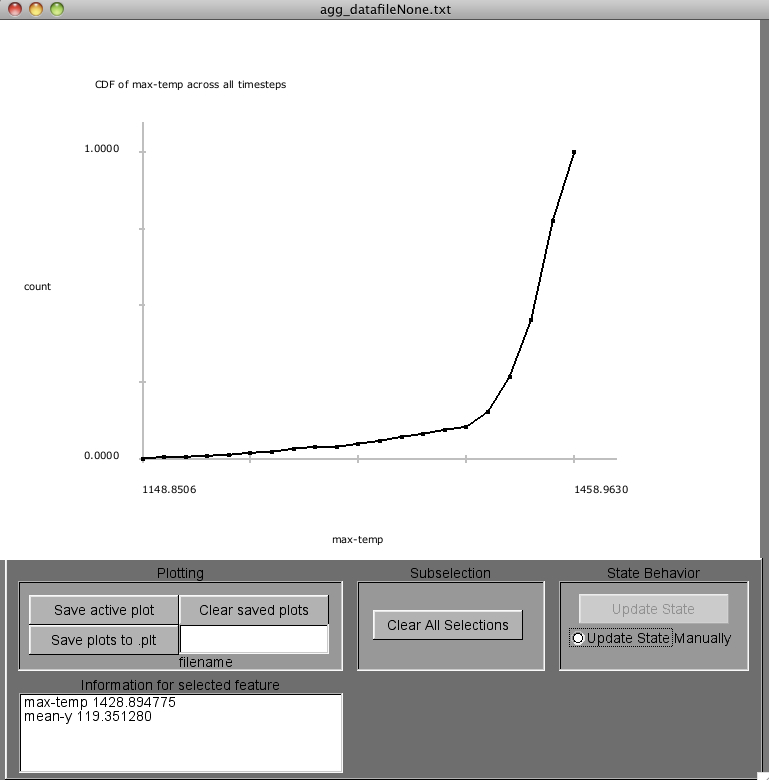
\includegraphics[width=6in]{jpeg/statsBrowser.jpg} 
  \caption{The plot display window for the Statistics Browser.  Buttons are used to save and clear
    active plots, clear sub-selected feature ids and save plots in gnuplot format. By default
  the plot browser is automatically updated according to changes in the Flexble GUI, however an 
  option is provided which allows the user to manually update the plot state after a set of multiple
  changes has been made.  This option can be useful when working with large data sets.}
  \label{fig:statsBrowser}
\end{figure}


Note that statistical plots can also be generated in batch mode using
\texttt{./utilities/batchExplorer} and can be generated via an interactive
command line setting using \texttt{./utilities/commandLineProc}. To get help with
either of these options type \texttt{--help} after the program name to get a list of usage
options.  As with the Statistics Browser, you can specify a plot name and a gnuplot 
file (with a .plt extension) will be generated with associated data files stored in 
.dat files.  

\paragraph{Segmentation Viewer} 
The Segmentation viewer is used to visualize the feature segmentation stored in the segmentation files.
To run the segmentation viewer type the following at a command prompt:

{\footnotesize
\texttt{\%./SegmentationViewer <first time> <last time> <family template> <segmentation template> <map template> dx dy dz <optional threshold>}
}


The following is an example call (with the optional threshold specified as 12.0):

{\footnotesize \texttt{
\%./SegmentationViewer 1000 1090 10 data\_\%d.family data\_\%d.seg data\_\%d.map 256 256 768 12.0
  }}

The segmentation viewer has a set of sliders that can be used to specify threshold and timestep, see figure 
\ref{fig:segViewer} and figure \ref{fig:segViewerControls}.  There are some sliders that can be used to cache a set of timesteps for a more interactive 
experience with large data sets. By default segmentations are not loaded automatically as the state changes, rather
you must press the load segmentation button with each change of state or check the autoload segmentations checkbox
load them automatically.  

A final feature of the segmentation viewer is that it can be synchronized with the statistics browser.  Details on
this are found below.

\begin{figure}[h]
  \center
  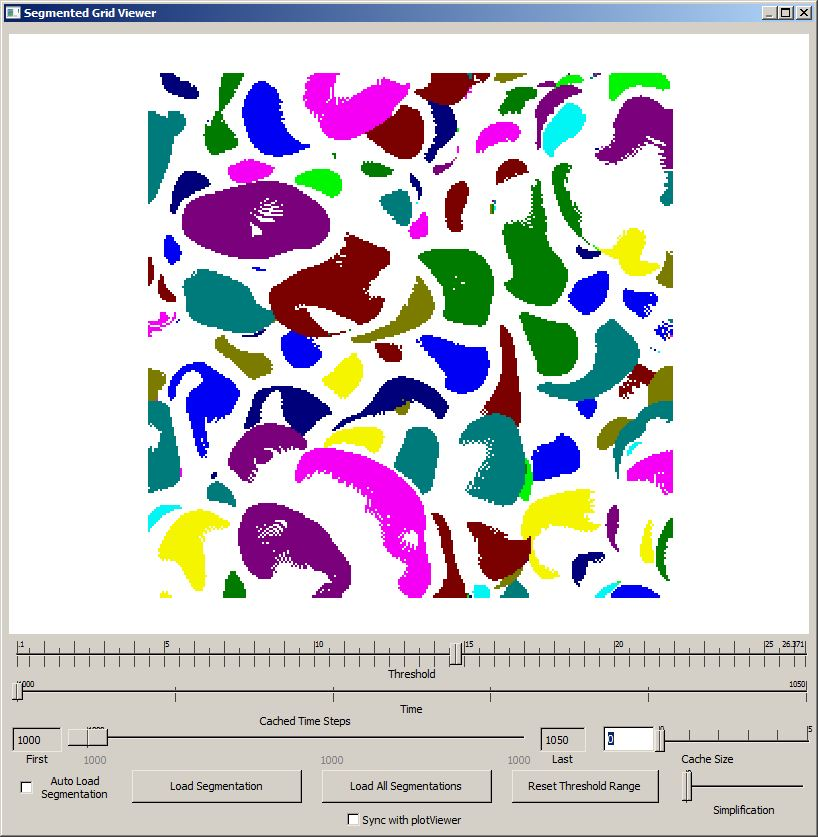
\includegraphics[width=6in]{jpeg/segViewer.jpg} 
  \caption{The segmentation viewer visualizes feature segments.  It comes with its own sliders to control the current view, or it
  can be synchronized to run using the conrols from the Flexible GUI of the Statistics browser.}
  \label{fig:segViewer}
\end{figure}

\begin{figure}[h]
  \center
  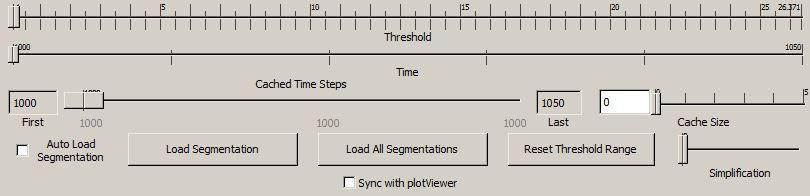
\includegraphics[width=6in]{jpeg/segViewerSliders.jpg} 
  \caption{The controls provided by the SegViewer. The sliders provide for control over the currently viewed data as well as utility controls to enable smoother interaction.}
  \label{fig:segViewerControls}
\end{figure}

\paragraph{Synchronizing the Statistics Browser and Segmentation Viewer}
When the Sync with plot viewer checkbox is selected in the Segmentation Viewer GUI, the state of the Segmentation Viewer
is controlled via the Flexible GUI controls in the Statistcs Browser.   To use this feature, the Statistics Browser and Segmentation viewer must be 
installed and run from the same directory as their communication is performed via a set of shared files. Simply start the Segmentation viewer and the
Statistics browser as specified above and check the sync with plot viewer checkbox in the Segmentation Viwer GUI to synchronize these two viewers.


Synchronizing the Statistics Browser and Segmentation Viewer introduces several new mechanisms for exploring the data:
\begin{itemize}
\item Selection of a feature in the Segmentation Viewer (pressing Left-Shift and clicking with the mouse) will cause the loaded attributes 
associated with this feature to be listed in a text box in the Statistics Browser. 
\item Subselection sliders in the Flexible GUI can be used to subselect the data.  Each pair of min/max sliders can be used to modify the active 
range o a feature-attribute.  Only those features that are active (i.e. whose attributes all fall within the user-prescribed ranges) are
displayed in the Segmenation Viewer and used to compute the plots in the Statistics Browser.
\item Buckets in the histogram and CDF plots can be selected/deselected by clicking the mouse button on the screen in the are under the plotted curve.  
This will cause only those features that have contributed to that bucket to be drawn in the Segmentation Viewer.  Note that by default, plots are 
accumulated across all timesteps and clicking an a bucket will only display those segments in the Segmentation Viewer that have contributed from 
the activetimestep.  If you want, you can click the “restrictComputationsToActiveTimestep” checkbox and the plot will be computed using data from 
the active timestep only.
\end{itemize}

\begin{figure}[h]
  \center
  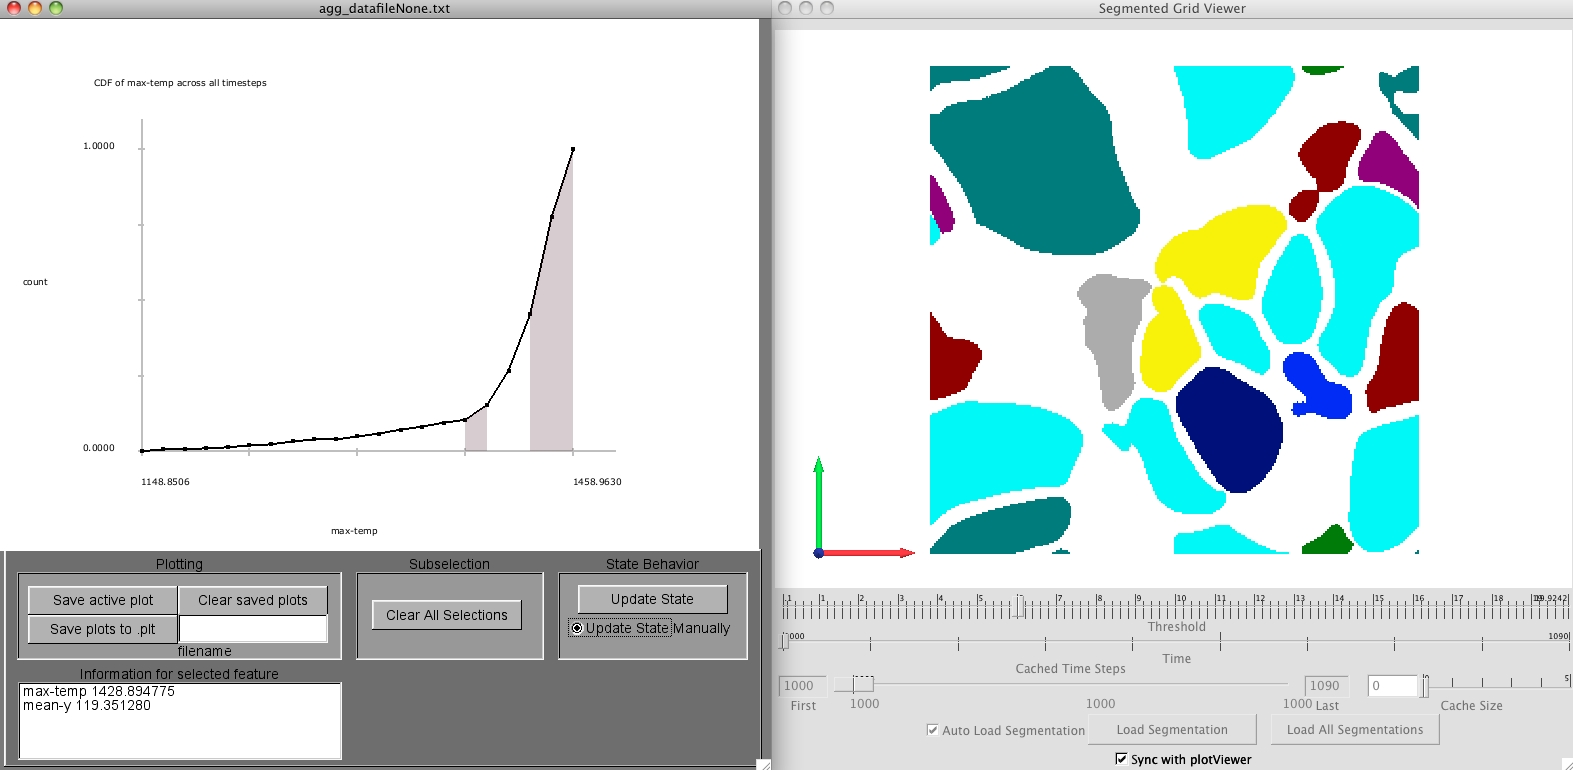
\includegraphics[width=6in]{jpeg/plotSelection.jpg} 
  \caption{The grey feature in the Segmentation Viewer is selected, and the data associated with this feature is displayed in the window in the 
 lower left hand corner of the Statistics Browser.  Several buckets in the CDF are selected and only those features who contribute to those buckets are displayed
 in the Segmentation Viewer. } 
  \label{fig:statsBrowser}
\end{figure}


\paragraph{Merge Tree Viewer}
